\documentclass[reqno]{../../../Projects/LaTeX/gtpart}

% \kern-1em % negative \quad.
% \kern-2em % negative \qquad.

\usepackage{minted}
\usepackage[scale=1.5,externalize=0]{strands}

\title[Strands package]{Strands package\\{\tt strands.sty}}

\author[D. Arcis]{Diego Arcis}
\address{FACSA, Universidad Aut\'onoma de Chile - Sede Talca, 5 Poniente 1670, Talca 3460000, Chile.}
\email{diego.arcis@uautonoma.cl}

%\subject{primary}{msc2010}{05A18}

\numberwithin{equation}{section}

\begin{document}

\maketitle

In case the package is already installed or if the {\tt strands.sty} file lies in the same folder as the main {\tt *tex} file, then it is used as usual:
\begin{minted}{latex}
	\usepackage[<options>]{strands}
\end{minted}
Otherwise, {\tt strands} should be complemented with the location of the {\tt *.sty} file. 

It is worth to mention that the Strands package will call the following additional packages: {\tt forarray}, {\tt ifthen}, {\tt tikz}, {\tt xfp}, {\tt xstring} and {\tt xkeyval}.

\section{The \mintinline{latex}{\vpartition} macro}

Use the macro \mintinline{latex}{\vpartition} to draw a set partition in the partition monoid as\[\mintinline{latex}{\vpartition[<options>]{<sorted blocks>}}\]where \mintinline{latex}{<sorted blocks>} are the blocks, separated by commas, entered as blocks of a set partition of $\{\pm1,\ldots,\pm n\}$. The positive numbers correspond to the dots above and the negative numbers correspond to the dots below. For instance:\[\begin{array}{c}
\vpartition{{1,3,-3,-4,-6},{6,5,-5,-2},{-1,2}}\\
%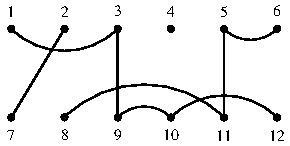
\includegraphics{pics/000.pdf}\\
\mintinline{latex}{\vpartition{{1,3,-3,-4,-6},{6,5,-5,-2},{-1,2}}}
\end{array}\]Note that the dots are connected in the order as the numbers appear on the blocks. So, if we change the position of numbers it will output a different representation.

The options \mintinline{latex}{<options>} are entered as \mintinline{latex}{<option>=<value>} and defined as follows:
\begin{itemize}
\item \mintinline{latex}{bend}: Integer number to manage the bend of brackets. Default value is $45$.
\item \mintinline{latex}{bulla}: Use $1$ to draw bullets from $1$ to $n$ above, otherwise use $0$. Default value is $1$.
\item \mintinline{latex}{bullb}: Use $1$ to draw bullets from $-1$ to $-n$ below, otherwise use $0$. Default value is $1$.
\item \mintinline{latex}{bulletends}: Float number to manage the size of the bullets. Default value is $0.04$.
\item \mintinline{latex}{floor}: Nonnegative float number setting where the picture starts to be drawn. So it starts at \mintinline{latex}{floor}$*$\mintinline{latex}{height}. Default value is $0$.
\item \mintinline{latex}{font}: Nonnegative float number setting the size of the font labelling the dots. Default value is $0.7$.
\item \mintinline{latex}{height}: Positive float number setting the height of the picture. Default value is $1$. 
\item \mintinline{latex}{labelver}: Space between dots and labels. Default value is $0.2$.
\item \mintinline{latex}{labelhor}: Additional space between labels (only for signed labels). Default value is $0.03$.
\item \mintinline{latex}{norma}: Positive float number to normalize the height above \mintinline{latex}{floor} with other pictures. Default value is $0$.
\item \mintinline{latex}{normb}: Negative float number to normalize the height below \mintinline{latex}{floor} with other pictures. Default value is $0$.
\item \mintinline{latex}{nstr}: Positive integer defining the number of strands. This value is used only if it is bigger than the self computed value.
\item \mintinline{latex}{reflect}: Use $1$ to mirror the brackets connections vertically, otherwise use $0$. Default value is $0$.  
\item \mintinline{latex}{rotate}: Integer number to rotate the picture. Default value is $0$. It cannot be used with the \mintinline{latex}{tkzpic}=1 option.
\item \mintinline{latex}{scale}: Positive float number to scale the picture. Default value is $1$. It cannot be used with the \mintinline{latex}{tkzpic}=1 option.
\item \mintinline{latex}{strwidth}: Positive float number to set the width of the strands. Default value is $0.7$.
\item \mintinline{latex}{tkzpic}: Use $1$ to add the \mintinline{latex}{tikzpicture} environment automatically, otherwise use $0$. Default value is $1$. Note that options \mintinline{latex}{rotate} and \mintinline{latex}{scale} will not work if \mintinline{latex}{tkzpic} is $0$ and they should be set with the environment.
\item \mintinline{latex}{type}: Number in $\{0,\pm1,2,\pm3,\pm4,5\}$ to set the labels of the dots. Default value is $3$. Each number is defined as follows:\begin{enumerate}
\item[(0)] Use $0$ to put no labels.
\item[(2)] Use $2$ to put labels from $1$ to $n$ above and below and use $1$ or $-1$ to remove the labels below or above respectively.
\item[(3)]Use $3$ to put labels from $1$ to $n$ above and labels from $n+1$ to $2n$ below. Use $-3$ to remove the labels above.
\item[(4)]Use $4$ to put labels from $1$ to $n$ above and labels from $1'$ to $n'$ below. Use $-4$ to remove the labels above.
\item[(5)]Use $5$ to put signed labels from $-n$ to $n$ with $n$ an even number.
\end{enumerate}
\item \mintinline{latex}{width}: Positive float number to set the width between horizontal dots. Default value is $0.6$.
\end{itemize}
Most of the options defined above can be set as global options in the \mintinline{latex}{\usepackage} macro, these are: {\tt bend}, {\tt bulletends} (as {\tt bulletsize}), {\tt font}, {\tt height}, {\tt labelhor}, {\tt labelver}, {\tt norma}, {\tt normb}, {\tt nstr}, {\tt rotate}, {\tt scale}, {\tt strwidth}, {\tt tkzpic} and {\tt width}.

Below a more complex example:\[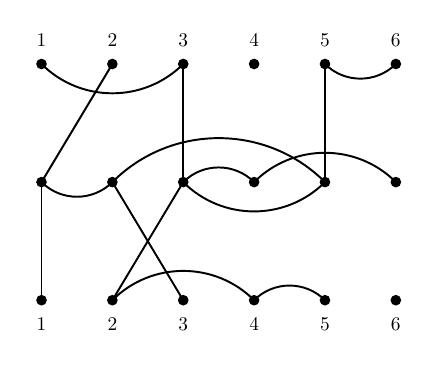
\begin{tikzpicture}[scale=1.5]
\vpartition[
	bullb=0,
	floor=1,
	tkzpic=0,
	type=1
]{{1,3,-3,-4,-6},{6,5,-5,-2},{-1,2}}
\vpartition[
	nstr=6,
	tkzpic=0,
	type=-1
]{{-1,1,2,-3},{5,3,-2,-4,-5}}
\end{tikzpicture}
%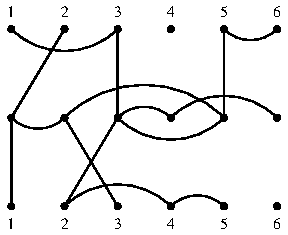
\includegraphics{pics/001.pdf}
\]

\begin{minted}{latex}
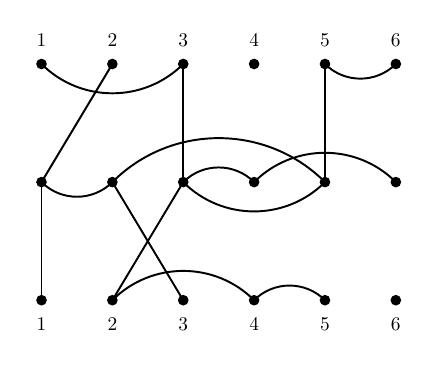
\begin{tikzpicture}[scale=1.5]
	\vpartition[
		bullb=0,
		floor=1,
		tkzpic=0,
		type=1
	]{{1,3,-3,-4,-6},{6,5,-5,-2},{-1,2}}
	\vpartition[
		nstr=6,
		tkzpic=0,
		type=-1
	]{{-1,1,2,-3},{5,3,-2,-4,-5}}
\end{tikzpicture}
\end{minted}

\subsection{The \mintinline{latex}{\arcpartition} macro}

Use the macro \mintinline{latex}{\arcpartition} to draw the graph of a set partition of $\{1,\ldots,n\}$ as\[\mintinline{latex}{\arcpartition[<options>]{<sorted blocks>}}\]where \mintinline{latex}{<sorted blocks>} are the blocks, separated by commas. This macro is constructed from \mintinline{latex}{\vpartition}, so its behavior is similar. For instance:\[\begin{array}{c}
\arcpartition{{1,4},{2,3,7}}\\
%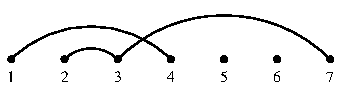
\includegraphics{pics/002.pdf}\\
\mintinline{latex}{\arcpartition{{1,4},{2,3,7}}}
\end{array}\]

The options \mintinline{latex}{<options>} come from \mintinline{latex}{\vpartition}, so most of them are defined in the same way, these are: \mintinline{latex}{bend}, \mintinline{latex}{floor}, \mintinline{latex}{font}, \mintinline{latex}{labelver}, \mintinline{latex}{lavelhor}, \mintinline{latex}{norma}, \mintinline{latex}{normb}, \mintinline{latex}{rotate}, \mintinline{latex}{scale}, \mintinline{latex}{strwidth}, \mintinline{latex}{tkzpic} and \mintinline{latex}{width}. However, the following options work different:
\begin{itemize}
\item \mintinline{latex}{bull}: Use $1$ to draw bullets from $1$ to $n$. Otherwise use $0$. Default value is $1$.
\item \mintinline{latex}{bulletsize}: Float number to manage the size of the bullets. Default value is $0.04$.
\item \mintinline{latex}{num}: Positive integer defining the number of dots. This value is used only if it is bigger than the self computed value.
\item \mintinline{latex}{type}: Use $1$ to put labels from $1$ to $n$, otherwise use $0$. Default value is $1$.
\end{itemize}
Most of the options can be set as global options in the \mintinline{latex}{\usepackage} macro, these are: {\tt bend}, {\tt bulletsize}, {\tt font}, {\tt labelhor}, {\tt labelver}, {\tt norma}, {\tt normb}, {\tt num}, {\tt rotate}, {\tt scale}, {\tt strwidth}, {\tt tkzpic} and {\tt width}.

\subsection{The \mintinline{latex}{\permutation} macro}

Use the macro \mintinline{latex}{\permutation} to draw permutations in the partition monoid as\[\mintinline{latex}{\permutation[<options>]{<permutation images>}}\]where \mintinline{latex}{<permutation images>} is the list of images of $1$ to $n$ under the permutation, separated by commas. This macro is constructed from \mintinline{latex}{\vpartition}, so its behavior is similar. For instance:\[\begin{array}{c}
\permutation{3,1,4,5,2}\\
%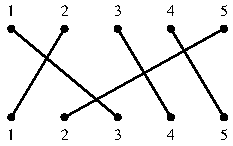
\includegraphics{pics/003.pdf}\\
\mintinline{latex}{\permutation{3,1,4,5,2}}
\end{array}\]

The options \mintinline{latex}{<options>} come from \mintinline{latex}{\vpartition}, so they are defined in the same way, these are: \mintinline{latex}{bulla}, \mintinline{latex}{bullb}, \mintinline{latex}{bulletends}, \mintinline{latex}{floor}, \mintinline{latex}{font}, \mintinline{latex}{height}, \mintinline{latex}{labelver}, \mintinline{latex}{lavelhor}, \mintinline{latex}{norma}, \mintinline{latex}{normb}, \mintinline{latex}{nstr}, \mintinline{latex}{rotate}, \mintinline{latex}{scale}, \mintinline{latex}{strwidth}, \mintinline{latex}{tkzpic}, \mintinline{latex}{type} and \mintinline{latex}{width}.

Most of the options defined above can be set as global options in the \mintinline{latex}{\usepackage} macro, these are: {\tt bulletends} (as {\tt bulletsize}), {\tt font}, {\tt height}, {\tt labelhor}, {\tt labelver}, {\tt norma}, {\tt normb}, {\tt nstr}, {\tt rotate}, {\tt scale}, {\tt strwidth}, {\tt tkzpic} and {\tt width}.

\subsection{The \mintinline{latex}{\tiedpair} macro}

Use the macro \mintinline{latex}{\tiedpair} to draw a permutation with a set partition of $[n]$ above as\[\mintinline{latex}{\tiedpair{<permutation>}{<set partition>}}\]where \mintinline{latex}{<permutation>} works as in \mintinline{latex}{\permutation} and \mintinline{latex}{<set partition>} works as in \mintinline{latex}{\arcpartition} macro. This macro is constructed from the mentioned ones, so its behavior is similar. For instance:\[\begin{array}{c}
\tiedpair{2,1,4,6,7,3,5}{{1,4,5},{3,6,7}}\\
%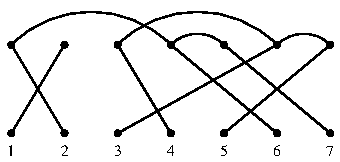
\includegraphics{pics/004.pdf}\\
\mintinline{latex}{\tiedpair{2,1,4,6,7,3,5}{{1,4,5},{3,6,7}}}
\end{array}\]

The options \mintinline{latex}{<options>} come from \mintinline{latex}{\vpartition}, so they are defined in the same way, these are: \mintinline{latex}{bend}, \mintinline{latex}{bulla}, \mintinline{latex}{bullb}, \mintinline{latex}{bulletends}, \mintinline{latex}{floor}, \mintinline{latex}{font}, \mintinline{latex}{height}, \mintinline{latex}{labelver}, \mintinline{latex}{lavelhor}, \mintinline{latex}{norma}, \mintinline{latex}{normb}, \mintinline{latex}{nstr}, \mintinline{latex}{rotate}, \mintinline{latex}{scale}, \mintinline{latex}{strwidth}, \mintinline{latex}{tkzpic}, \mintinline{latex}{type} and \mintinline{latex}{width}. However, there is an additional option named \mintinline{latex}{above} which is $1$ by default and can be changed to $0$ to put the set partition below.

Most of the options defined above can be set as global options in the \mintinline{latex}{\usepackage} macro, these are: {\tt bend}, {\tt bulletends} (as {\tt bulletsize}), {\tt font}, {\tt height}, {\tt labelhor}, {\tt labelver}, {\tt norma}, {\tt normb}, {\tt nstr}, {\tt rotate}, {\tt scale}, {\tt strwidth}, {\tt tkzpic} and {\tt width}.

\subsection{The \mintinline{latex}{\tie} macro}

Use the macro \mintinline{latex}{\tie} inside a \mintinline{latex}{tikzpicture} environment to draw a tie with some other pictures as\[\mintinline{latex}{\tie[<options>]{<dots>}}\]where \mintinline{latex}{<dots>} is the list of dots where this tie is connected. Each dot can be entered as a number $k$ defining the horizontal position inside the \mintinline{latex}{width} or as a pair $\{k,h\}$ where $h$ is its vertical position respect to \mintinline{latex}{height}. For instance:
\[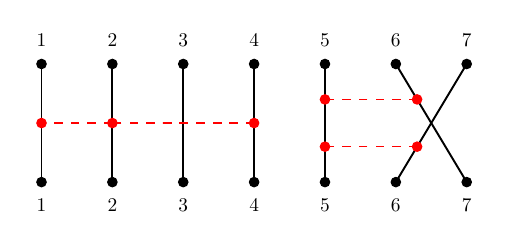
\begin{tikzpicture}[scale=1.5]
	\permutation[tkzpic=0]{1,2,3,4,5,7,6}
	\tie{1,2,4}
	\tie{{5,0.7},{6.3,0.7}}
	\tie{{5,0.3},{6.3,0.3}}
\end{tikzpicture}
%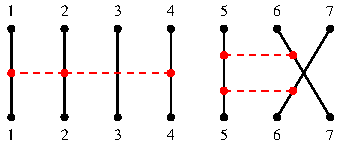
\includegraphics{pics/005.pdf}
\]

\begin{minted}{latex}
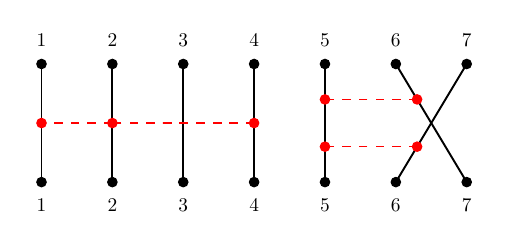
\begin{tikzpicture}[scale=1.5]
	\permutation[tkzpic=0]{1,2,3,4,5,7,6}
	\tie{1,2,4}
	\tie{{5,0.7},{6.3,0.7}}
	\tie{{5,0.3},{6.3,0.3}}
\end{tikzpicture}
\end{minted}

The options \mintinline{latex}{<options>} are defined as follows:
\begin{itemize}
\item \mintinline{latex}{bend}: Integer number to manage the bend of the tie. Default value is $0$.
\item \mintinline{latex}{bull}: Use $1$ to draw the connection bullets, otherwise use $0$. Default value is $1$.
\item \mintinline{latex}{bulletie}: Float number to manage the size of the bullets on ties. Default value is $0.04$.
\item \mintinline{latex}{color}: Set the color of the ties. Default value is \mintinline{latex}{red}.
\item \mintinline{latex}{floor}: Nonnegative float number setting where the main picture starts to be drawn. Default value is $0$.
\item \mintinline{latex}{height}: Positive float number setting the height of the main picture. Default value is $1$.
\item \mintinline{latex}{snake}: Use \mintinline{latex}{true} to set the snake style, otherwise use \mintinline{latex}{false}. Default value is \mintinline{latex}{false}.
\item \mintinline{latex}{snakeamp}: Set the amplitude of the snakes. Use with \mintinline{latex}{snake} option. Default value is $1$.
\item \mintinline{latex}{snakends}: Set the length of the snake ends. Use with \mintinline{latex}{snake} option. Default value is $0$.
\item \mintinline{latex}{snakelen}: Set the snake of each snake cycle. Use with \mintinline{latex}{snake} option. Default value is $3$.
\item \mintinline{latex}{style}: Set the style of the tie (\mintinline{latex}{solid}, \mintinline{latex}{dashed}, \mintinline{latex}{dotted}). Default value is \mintinline{latex}{dashed}.
\item \mintinline{latex}{tieheight}: Positive float number setting the vertical position of dots if these were entered as a single number. Default value is $0.5$.
\item \mintinline{latex}{tiewidth}: Positive float number setting the width of the line representing a tie. Default value is $0.5$.
\item \mintinline{latex}{width}: Positive float number setting the width between horizontal dots of the main picture. Default value is $0.6$.
\end{itemize}Most of the options can be set as global options in the \mintinline{latex}{\usepackage} macro, these are: {\tt bend} (as {\tt tiebend}), {\tt bulletie} (as {\tt bulletsize}), {\tt color} (as {\tt tiecolor}), {\tt height}, {\tt snake} (as {\tt tiesnake}), {\tt snakeamp} (as {\tt tiesnakeamp}), {\tt snakends} (as {\tt tiesnakends}), {\tt snakelen} (as {\tt tiesnakelen}), {\tt style} (as {\tt tiestyle}), {\tt tieheight}, {\tt tiewidth} and {\tt width}.

\section{The \mintinline{latex}{\strands} macro}

Use the macro \mintinline{latex}{\strands} to draw braid-like objects as a product of generators as\[\mintinline{latex}{\strands[<options>]{<generators>}}\]where \mintinline{latex}{<generators>} is a list of generators \mintinline{latex}{ai} separated by elements in $\{*,-\}$. Use $*$ to put the next generator in the following floor and $-$ otherwise. For instance:\[\begin{array}{c}
\strands{p1-n3-e5*v2-t4-f6*s1-n3-p6*n1-e3-s5}\\
%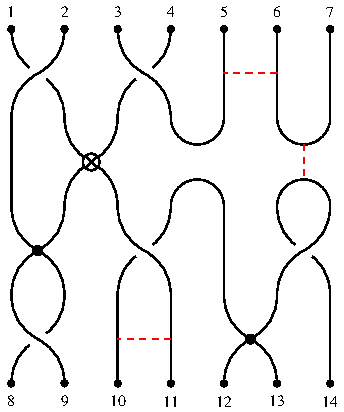
\includegraphics{pics/006.pdf}\\
\mintinline{latex}{\strands{p1-n3-e5*v2-t4-f6*s1-n3-p6*n1-e3-s5}}
\end{array}\]See a more complex picture at the end of this section. Note that it is used is similar to the known Braid Package but with different options.

The characters defining each type of generator can be changed in the \mintinline{latex}{\usepackage} macro:\begin{itemize}
\item \mintinline{latex}{gencharposbraid}: Classic positive braid generator. Default value is p.
\item \mintinline{latex}{gencharnegbraid}: Classic negative braid generator. Default value is n.
\item \mintinline{latex}{gencharvirtual}: Virtual braid generator. Default value is v.
\item \mintinline{latex}{gencharsingular}: Singular braid generator. Default value is s.
\item \mintinline{latex}{genchartangle}: Tangle generator. Default value is t.
\item \mintinline{latex}{genchartie}: Tie generator. Default value is e.
\item \mintinline{latex}{genchartiedtangle}: Tied tangle generator. Default value is f.
\item \mintinline{latex}{genchartrivial}: Trivial generator or identity. Default value is i.
\end{itemize}

The options \mintinline{latex}{<options>} for this macro are defined as follows:
\begin{itemize}
\item \mintinline{latex}{bendbraid}: Manage the bend of the braid generators.
\item \mintinline{latex}{bendtangle}: Manage the bend of the tangle generators.
\item \mintinline{latex}{bulla}: Use $1$ to draw the bullets above, otherwise use $0$.
\item \mintinline{latex}{bullb}: Use $1$ to draw the bullets below, otherwise use $0$.
\item \mintinline{latex}{bulletends}: Float number to manage the size of the bullets. Default value is $0.04$.
\item \mintinline{latex}{direction}: Direction in which the generators appear. Default is $1$.
\item \mintinline{latex}{floor}: Manage the floor where the picture starts.
\item \mintinline{latex}{font}: Manage the font of the labels.
\item \mintinline{latex}{height}: Height of the picture.
\item \mintinline{latex}{labelhor}: Additional horizontal space between labels.
\item \mintinline{latex}{labelver}: Vertical space between labels and bullets.
\item \mintinline{latex}{nstr}: Number of strands.
\item \mintinline{latex}{rotate}: Rotate angle of the picture.
\item \mintinline{latex}{scale}: Scale the picture.
\item \mintinline{latex}{strwidth}: Width of the strands.
\item \mintinline{latex}{tiebull}: Use $1$ to put bullets on ties ends, otherwise use $0$. Default value is $0$.
\item \mintinline{latex}{tiebullsize}: Float number to manage the size of the bullets on ties. Default value is $0.04$.
\item \mintinline{latex}{tiecolor}: Manage the color of the ties. Default value is \mintinline{latex}{red}.
\item \mintinline{latex}{tieheight}: Manage the vertical position of ties respect to each generator.
\item \mintinline{latex}{tiesnake}: Use \mintinline{latex}{true} to snake the ties, otherwise use \mintinline{latex}{false}. Default value is false.
\item \mintinline{latex}{tiesnakeamp}: Manage the amplitude of the snakes.
\item \mintinline{latex}{tiesnakends}: Length of the ends of snakes.
\item \mintinline{latex}{tiesnakelen}: Length of snakes cycles.
\item \mintinline{latex}{tiestyle}: Manage the style of ties (\mintinline{latex}{solid},\mintinline{latex}{dashed},\mintinline{latex}{dotted}). Default value is \mintinline{latex}{dashed}.
\item \mintinline{latex}{tiewidth}: Width of the ties.
\item \mintinline{latex}{tkzpic}: Use $1$ to add the \mintinline{latex}{tikzpicture} environment automatically, otherwise use $0$. Default value is $1$.
\item \mintinline{latex}{type}: Manage the type of labels as in \mintinline{latex}{\vpartition}.
\item \mintinline{latex}{width}: Width between dots.
\end{itemize}Most of the options can be set as global options in the \mintinline{latex}{\usepackage} macro, these are: {\tt bendbraid}, {\tt bendtangle}, {\tt bulletends} (as {\tt bulletsize}), {\tt direction}, {\tt font}, {\tt height}, {\tt labelver}, {\tt labelhor}, {\tt rotate}, {\tt scale}, {\tt strwidth}, {\tt tiebull}, {\tt tiebullsize}, {\tt tiecolor}, {\tt tieheight}, {\tt tiesnake}, {\tt tiesnakeamp}, {\tt tiesnakends}, {\tt tiesnakelen}, {\tt tiestyle}, {\tt tiewidth}, {\tt tkzpic} and {\tt width}.

Here another example:
\[\strands[
	rotate=90,
	tiesnake=true,
	tiesnakeamp=2,
	tiesnakelen=4,
	tiestyle=solid,
	type=2
]{p1-n3-e5*v2-t4-f6*s1-n3-p6*n1-e3-s5}
%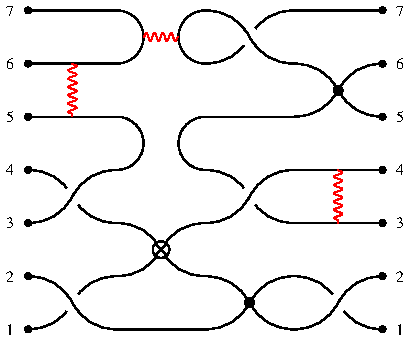
\includegraphics{pics/007.pdf}
\]
\begin{minted}{latex}
\strands[
	rotate=90,
	tiesnake=true,
	tiesnakeamp=2,
	tiesnakelen=4,
	tiestyle=solid,
	type=2
]{p1-n3-e5*v2-t4-f6*s1-n3-p6*n1-e3-s5}
\end{minted}

\section{More global options}

Here the global options that are not managed locally from the macros above. 
\begin{itemize}
\item {\tt backcolor}: This option must be always set as the color of the background or as the color of the paper in case it will be printed. Default value is {\tt white}.
\item {\tt braidcross}: Float number to set the size of the braid crossing. Default value is $3$.
\item {\tt braidsingcross}: Float number to set the size of the singular braid crossing. Default value is $1.6$.
\item {\tt braidvirtcross}: Float number to set the size of the virtual braid crossing. Default value is $8$.
\item {\tt coverunion}: This value should be increased if there is some white space between the floors. Default value is $0.001$.
\item {\tt externalize}: Use 1 to transform all tikz pictures into PDF files. Default value is $0$.
\item {\tt normcolor}: Color of a symbol used to normalize the height of pictures. Default value is {\tt transparent}.
\item {\tt normsymbo}: Symbol used to normalize the height of pictures. Default value is a dash: {\tt -}.
\item {\tt timeswidth}: Number of times the background is thickness. Default value is $3$.
\end{itemize}

\subsubsection*{Acknowledgements}
The author is part of the research group GEMA Res.180/2019 VRIP--UA and was supported, in part, by the grant Fondo Apoyo a la Investigaci\'on DIUA179-2020.

\bibliographystyle{plainurl}
\bibliography{../../../Projects/LaTeX/bibtex}

\end{document}